\documentclass[text.tex]{subfiles}

\begin{document}
\pagestyle{plain}
\section{Generation of a finite section of a quasicrystal with a general window}
Previous section concluded the analysis of a quasicrystal with a rhombic window. Now the results are applied to the analysis of quasicrystals with a window of a general shape. 

Once again first an algorithm for generating a finite section of a quasicrystal with a general window is presented.

A property from Remark \ref{rem:quasiProperties} (Theorem \ref{the:quasiProperties}) is a key to such algorithm:
$$\Omega \subset \tilde{\Omega} \Rightarrow \quasi{\Omega} \subset \quasi{\tilde{\Omega}}$$
To given general window $\Omega$ a rhombus window $\widehat{\Omega}$ is circumscribed. Therefore $\Omega\subset\widehat{\Omega}$. Such window $\widehat{\Omega}$ is called the hyper-window and the quasicrystal $\quasi{\widehat{\Omega}}$ is called the hyper-quasicrystal. 

Then a finite section of the hyper-quasicrystal $\quasi{\widehat{\Omega}}$ is constructed as described in previous sections and each point $x\in\quasi{\widehat{\Omega}}$ is individually tested whether $x^\ast\in\Omega$. Points that fail the test are discarded and the rest creates a finite section of the quasicrystal $\quasi{\Omega}$.

To illustrate the algorithm a special kind of quasicrystal is presented. It's window is in the shape of an \texttt{E} and it is called Eduard.
\begin{figure}[h!]
\centering
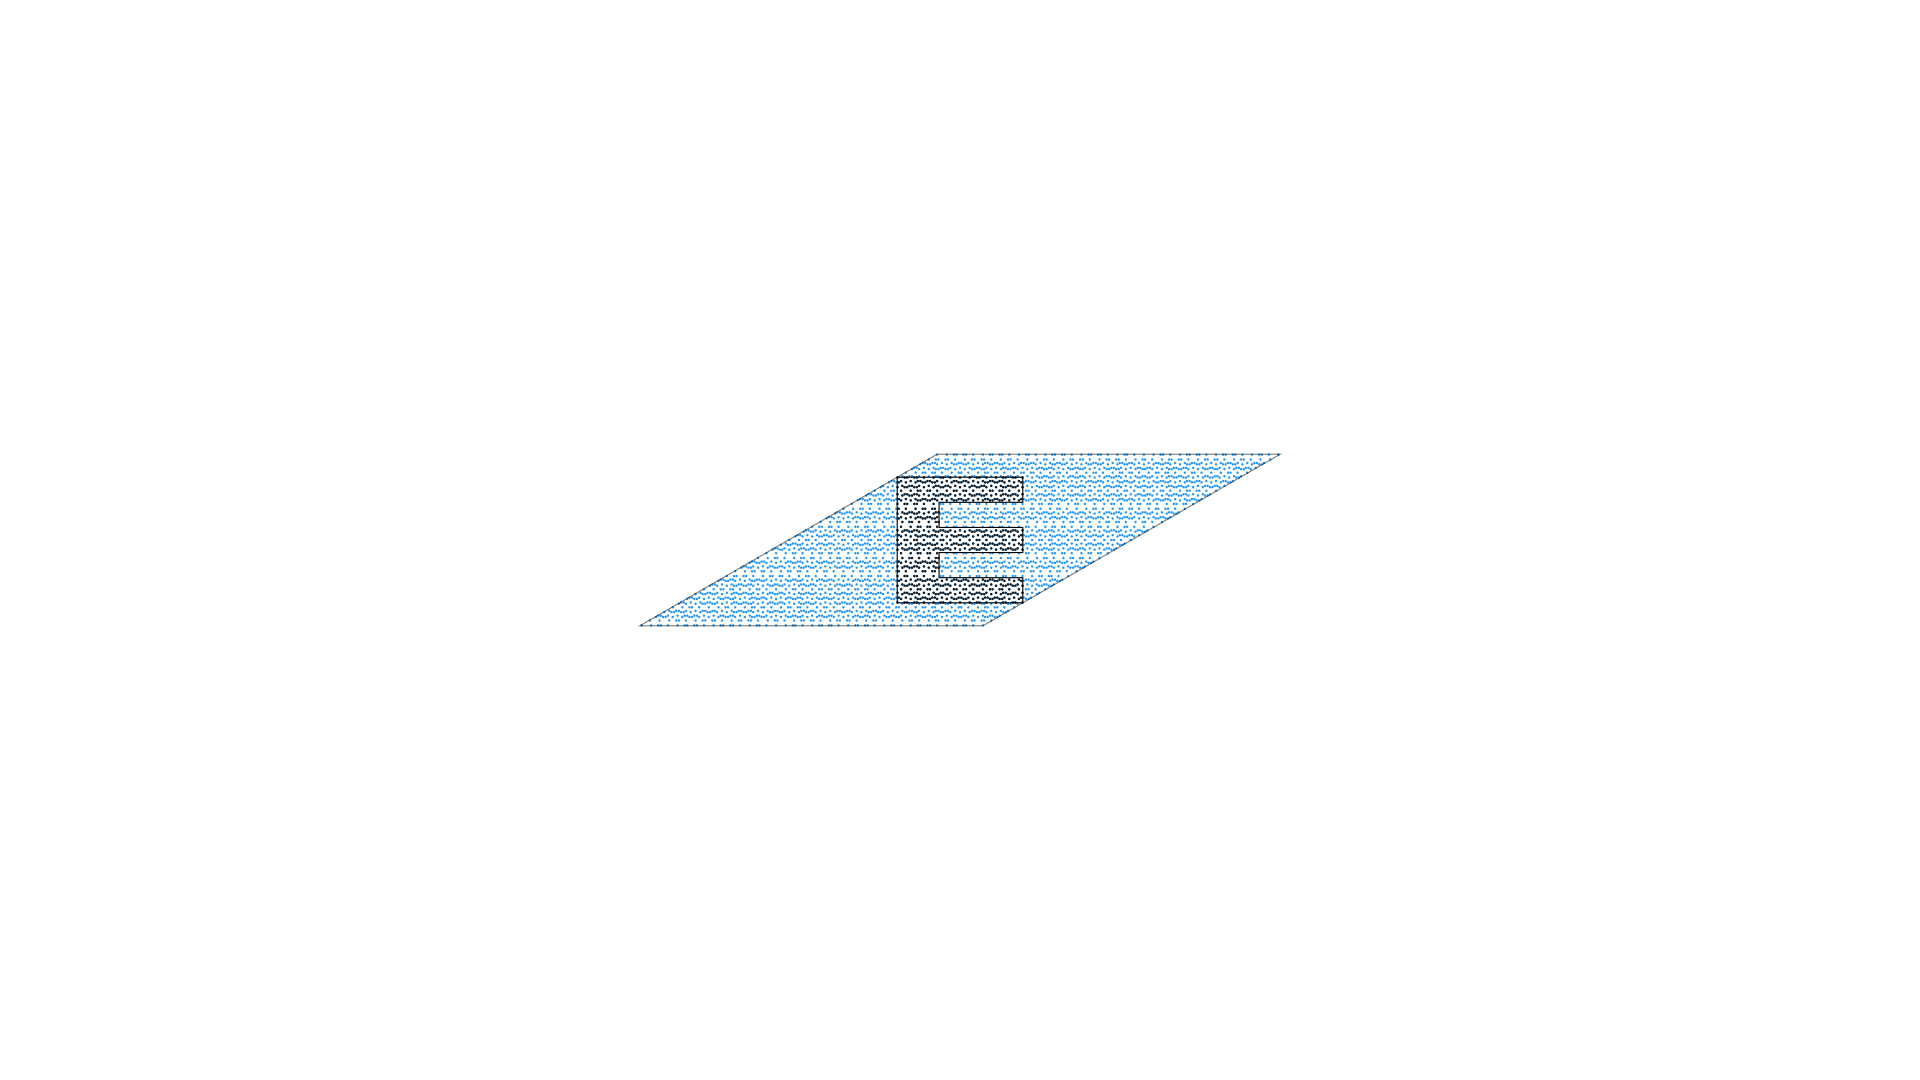
\includegraphics[width=1\textwidth]{the_eduard_window}
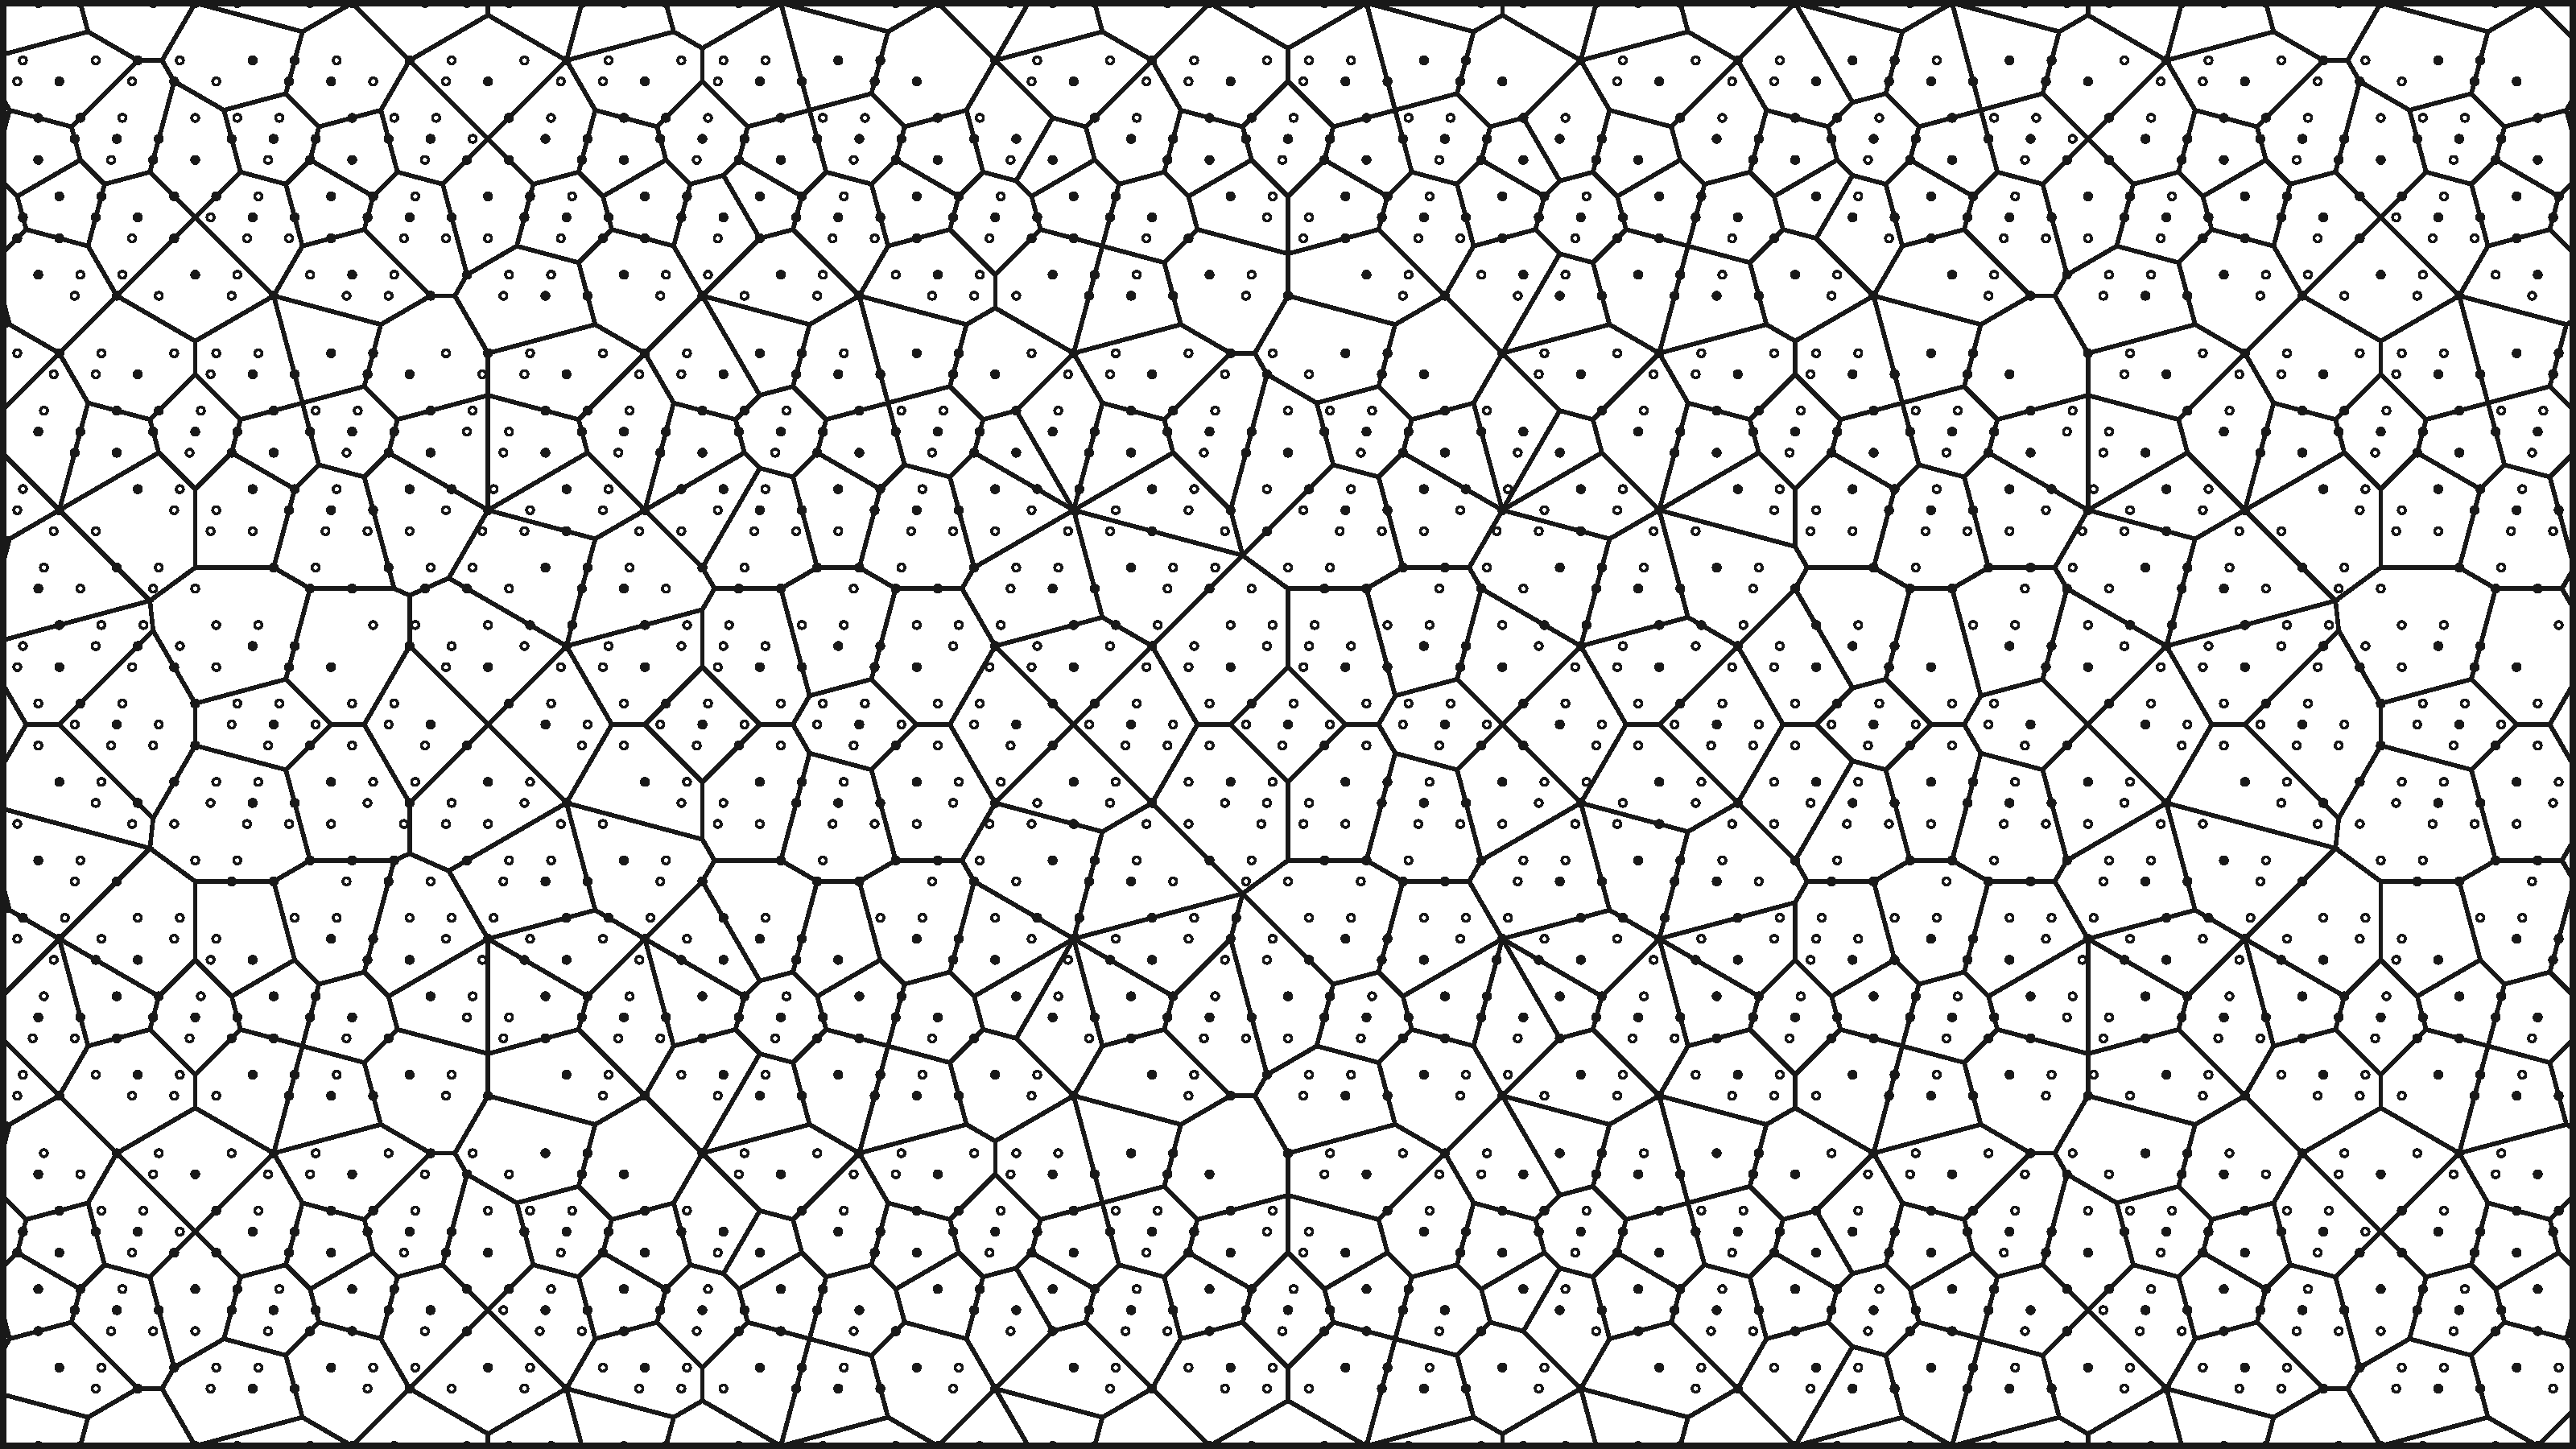
\includegraphics[width=1\textwidth]{the_eduard_quasi}
\caption{Illustration of the algorithm for generating a finite section of a quasicrystal with a general window. The top image displays a window in the shape of an \texttt{E} it's hyper-window and the $\ast$ images of points of the quasicrystal Eduard (full) and of points of the hyper-quasicrystal (empty). The lower image displays the quasicrystal Eduard (with voronoi polygons) and the hyper-quasicrystal (only points).}
\end{figure}

Such algorithm can be applied to a window of literally any shape as long as a rhombus can be circumscribed. The natural next step is to catalog all different voronoi polygons for all sizes of given general window. That is however significantly more complex than for a rhombic window.
\end{document}
